\subsection{Empfang von Daten}

Die Daten müssen auf beiden \ac{uC} ordnungsgemäß empfangen werden. Die Implementation unterscheidet sich hierbei stark. Der STM32 ermöglicht
die Nutzung seiner \ac{DMA}-Funktionalität, während auf dem ESP8266 eine Interruptbasierte Abfrage implementiert wird.


\subsubsection{STM32: Konfiguration des UART}
Wichtig bei der Konfiguration des \acp{UART} ist das Format und die Baudrate. Wie in \ref{sec:Grundlagen} erklärt, wird der \ac{UART} im 8N1-Modus
konfiguriert. Dies entspricht einer Nachrichtenlänge von acht Bit und keiner Parität. Die Geschwindigkeit wird auf 115200 Baud festgelegt (siehe Abb. \ref{img: Parameter}). 

\smallskip

Um die Nutzung des \ac{UART} in Kombination mit \ac{DMA} zu ermöglichen, muss der globale Interrupt
aktiviert werden. Der \ac{DMA} wird so konfiguriert, dass empfangsseitig die Daten direkt zum Speicher übertragen werden, während senderseitig die Daten
direkt vom Speicher zum \ac{UART} weitergeleitet werden. Zudem wird der Empfang von Daten per \ac{DMA} als Ringbuffer umgesetzt (siehe Abb. \ref{img: DMA}).


\begin{figure}[h]
    \centering
    \begin{subfigure}{0.45\textwidth}
        \centering
        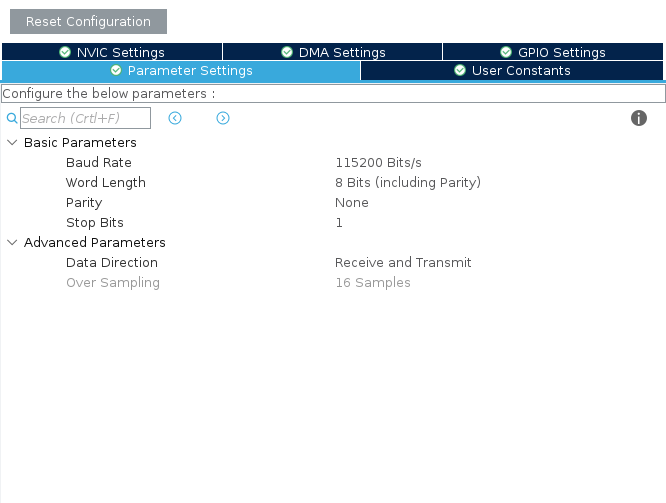
\includegraphics[width=\textwidth]{Pictures/parameter_uart.png}
        \caption{Baudrate,Format}
        \label{img: Parameter}
    \end{subfigure}
    %
    \begin{subfigure}{0.45\textwidth}
        \centering
        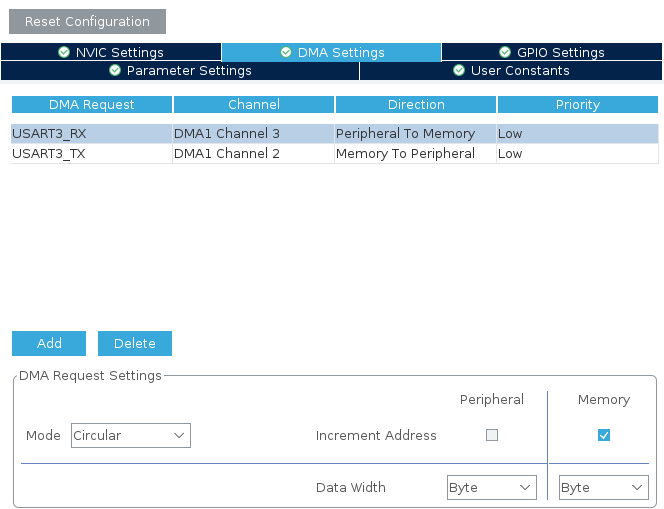
\includegraphics[width=\textwidth]{Pictures/dma_uart.png}
        \caption{DMA}
        \label{img: DMA}
    \end{subfigure}
    \caption{Konfiguration des \acp{UART}}
    \label{img: UART config}
  \end{figure}